\documentclass[a4paper,12pt]{article}
\addtolength{\oddsidemargin}{-1.cm}
\addtolength{\textwidth}{2cm}
\addtolength{\topmargin}{-3cm}
\addtolength{\textheight}{3.5cm}
\makeindex


\usepackage[pdftex]{graphicx}
\usepackage{makeidx}
\usepackage{float}
\usepackage{hyperref}
\hypersetup{
	colorlinks=true,
	linkcolor=blue,
	filecolor=magenta,      
	urlcolor=cyan,
}



% define the title
\author{CodeBlox}
\title{Tender}
\begin{document}
	\setlength{\parskip}{6pt}
	
	% generates the title
	\begin{titlepage}
		\begin{center}
			
\includegraphics[width=1\textwidth]{./Pictures/up_logo.png}\\[1.5cm] 
			\textsc{\LARGE Department of Computer Science} \\ [.5cm]
			\textsc{\Large Functional and Architectural Requirements} \\ [.5cm]
			\line(1,0){450}\\[.5cm]
			\huge{\bfseries Client: Gavin Potgieter}\\
			\line(1,0){450}\\[.5cm]
			\textsc{\LARGE Team: CodeBlox}\\ [0.5cm]
			
			
			\textsc{\large Tshepo Malesela (Bsc: Computer Science)}\\
			\textsc{\large Lethabo Mogase (Bsc: Computer Science)}\\
			\textsc{\large Lorenzo Spazzoli (Bsc: Computer Science)}\\
			\textsc{\large Bilal Muhammad (BIS: Multimedia)}\\
			\textsc{\large Dirk de Klerk (BIS: Multimedia)}\\ [3.9cm]
			
			\large\today
		\end{center}
	\end{titlepage}
	
	\tableofcontents
	\thispagestyle{empty}
	\footnotesize
	\normalsize
	
	
	
	
	\newpage
	\section{Introduction}
	The purpose of this document is to provide a detailed overview of the functional and architectural requirements with regard to the DropOff Project that was assigned to team CodeBlox. The document will be under constant revision, and will change as the project progresses. 
	
	{\noindent}It will provide the development team with a reference that can be used to develope from, thus ensuring that all functional and architectural requirements are met.
	
	{\noindent}The document will also serve as means of communication between the client and development team. Thus any additional requirements from the clients' side can be appended to the document, and has to be adhered to from the development side.
	
	\section{Project Objectives} The \textbf{primary objective} of the project is to create an automated service system that will provide customers with the ability to grant delivery personnel access to a drop safe and/or demarcated area of their home. This will ensure that deliveries to be made can be completed without the need of someone being physically present on the premises.
	
	{\noindent}Initially this will consist of the generation of a One Time Pin (OTP), that will be sent to the delivery personnel, granting them single access to the demarcated area. Once the delivery has been made. The user needs to be able to ensure that the residence is secure.
	
	{\noindent}If time allows it. The system will be expanded to use audio and video communication to validate the identity of the delivery person.
	
	{\noindent}In addition to the functionality of the system, it needs to be as \textbf{cost effective} as possible. This will allow a larger audience to gain access to the system. 
	
	{\noindent}The \textbf{secondary objective} (if time permits) is to make the system scalable. This will enable services to expand to other areas of the home. Thus allowing users an affordable solution to home automation.
	
	\newpage
	\section{Functional Requirements}
	
	\subsection{Users}
	The users module will be responsible for maintaining user information. Particularly it will specify what type of user it is. The module will also have the responsibility of storing demographic information about the users.
	
	\subsubsection{Scope}
	The scope of the Users module is shown below
	
	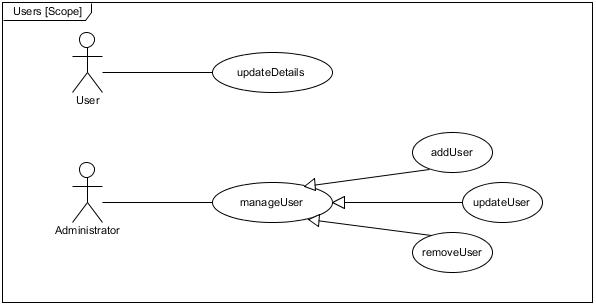
\includegraphics[width=1\textwidth]{./Pictures/UML/usersScope.jpg}\\[1.5cm]
	
	{\noindent}The scope of the Users module includes
	\begin{itemize}
		\item adding, removing, and modifying users on the system
		\item changing user information
	\end{itemize}
	
	\subsubsection{Domain Model}
	The domain model for the Users module is shown below
	
	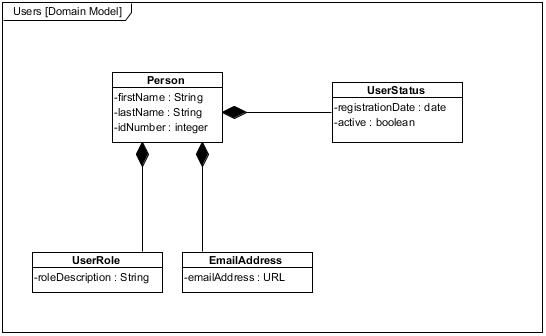
\includegraphics[width=1\textwidth]{./Pictures/UML/usersDomainModel.jpg}\\[1.5cm]	

	{\noindent}Each user has a firstname and a lastname, as well as an id number. The person will also have an email address associated with them that will be used for login purposes. Each person will also be associated with a role that will indicate if it is an administrator or general user. Lastly a status will be designated to each user to determine if they are active or not.	
	 
	\newpage
	\subsubsection{Use Cases}
	
	\begin{itemize}
		\item \textbf{addUser} - Allows an administrator to add a user to the system.\\[0.5cm]
		\textit{preconditions:}
			\begin{itemize}
				\item user does not already exist on the system
				\item creator possesses the role of administrator
			\end{itemize}
			
		\textit{postconditions:}
			\begin{itemize}
				\item a user is created.
				\item the user is added to the system.\\[0.5cm]
			\end{itemize}
			
		\item \textbf{removeUser} - Allows an administrator to remove a user to the system.\\[0.5cm]
		\textit{preconditions:}
			\begin{itemize}
				\item the user exists on the system
				\item remover possesses the role of administrator
			\end{itemize}
		
		\textit{postconditions:}
			\begin{itemize}
				\item a user is removed.
				\item the user is removed from the system.\\[0.5cm]
			\end{itemize}
			
		\item \textbf{updateUser} - Allows an administrator to modify a user on the system.\\[0.5cm]
		\textit{preconditions:}
			\begin{itemize}
				\item the user exists on the system
				\item modifier possesses the role of administrator
			\end{itemize}
		
		\textit{postconditions:}
			\begin{itemize}
				\item a users information is modified.\\[0.5cm]
			\end{itemize}
			
		\item \textbf{updateDetails} - Allows a general user to update their information.\\[0.5cm]
		\textit{preconditions:}
			\begin{itemize}
				\item the user exists on the system
				\item the user has to correct credentials
			\end{itemize}
		
		\textit{postconditions:}
			\begin{itemize}
				\item a users information is modified.
			\end{itemize}
	\end{itemize}
	
	\newpage
	\subsection{Controller}
	The controller module will be responsible for maintaining system status information as well as provide the various user with certain system functionalities depending on their authorization. Particularly it will specify the current status of the drop box/area and allow the user to change this status through specific functions. This module will also be responsible for generating the OTP.
	
	\subsubsection{Scope}
	The scope of the Controller module is shown below
	
	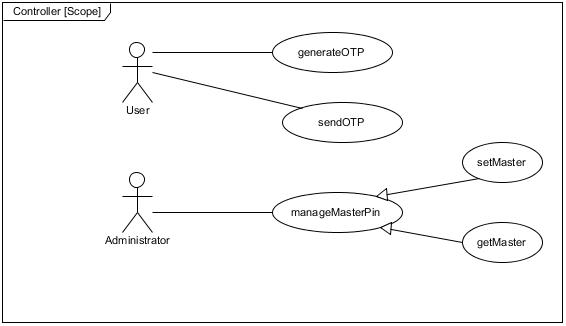
\includegraphics[width=1\textwidth]{./Pictures/UML/controllerScope.jpg}\\[1.5cm]
	
	{\noindent}The scope of the Users module includes
	\begin{itemize}
		\item generating, and sending an OTP.
		\item setting and getting a master pin (To be used as a fail safe).
		\item Users i.e. delivery person may request a OTP to access designated area.
	\end{itemize}
	
	\newpage
	\subsubsection{Domain Model}
	The domain model for the Controller module is shown below
	
	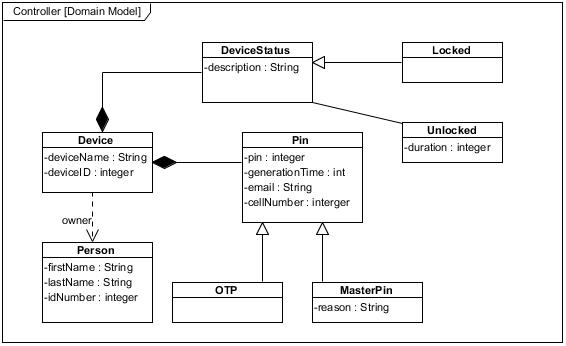
\includegraphics[width=1\textwidth]{./Pictures/UML/controllerDomainModel.jpg}\\[1.5cm]	
	
	{\noindent}The Device in this context will keep track of the status of a particular device connected to the system. Initially this device will refer to the drop safe or demarcated area within the house. Device will be a composite object consisting of a DeviceStatus and a Pin. The device will also be associated with a Person object which will be the owner of that particular device.\\
	
	{\noindent}\textbf{Person} refers to the owner of the device as stated earlier. Only one owner will be associated with each device at a particular time. This will serve the purpose of authenticating the owner so that an OTP may generated and sent to the requesting user/delivery person.\\
	
	{\noindent}\textbf{DeviceStatus} will indicate the current status of the device. This will be used as pre- and postconditions for the particular methods to be implemented. So far the device will possess to possible statuses: Locked or Unlocked. The \textbf{Unlocked} specialised class will have a textbf{duration} variable to set a time limit for when the system should lock up again after the demarcated area has been accessed.\\
	
	{\noindent}\textbf{Pin} will serve as a template for both the OTP and MasterPin. It will provide users with a primary means of access to the system. The Pin class possesses \textbf{email} and \textbf{cellNumber} variables that area the email and cell number of the delivery person to which a pin will be sent. Each Pin object will have a \textbf{generationTime} variable to indicate when a pin was generated. This will be used to set an expiry date for each pin as an extra precaution. 	
	
	\subsubsection{Use Cases}
	
	\begin{itemize}
		\item \textbf{generateOTP} - Allows an Owner to generate an OTP once they receive a requestOTP request from a User/delivery person.\\[0.5cm]
		\textit{preconditions:}
		\begin{itemize}
			\item The Owner received a requestOTP request from the delivery person.
			\item The Owner has authorization on the system.
		\end{itemize}
		
		\textit{postconditions:}
		\begin{itemize}
			\item An OTP is generated by the system.
			\item The OTP is registered on the system.\\[0.5cm]
		\end{itemize}
		
		\item \textbf{sendOTP} - Allows the Owner to send an OTP to a specific delivery person.\\[0.5cm]
		\textit{preconditions:}
		\begin{itemize}
			\item The OTP has been generated.
			\item The delivery person has been authorised to receive the OTP.
		\end{itemize}
		
		\textit{postconditions:}
		\begin{itemize}
			\item OTP is sent to the delivery person.\\[0.5cm]
		\end{itemize}
		
		\item \textbf{unlockDevice} - Allows the User/delivery person to unlock the demarcated area to make delivery.\\[0.5cm]
		\textit{preconditions:}
		\begin{itemize}
			\item The User possesses a valid OTP that can be matched against the systems OTP.
		\end{itemize}
		
		\textit{postconditions:}
		\begin{itemize}
			\item The System is unlocked and delivery can proceed.\\[0.5cm]
		\end{itemize}
		
		\item \textbf{requestOTP} - Allows the delivery person to request an OTP from the Owner of the residence.\\[0.5cm]
		\textit{preconditions:}
		\begin{itemize}
			\item The system is locked.
			\item A delivery has to be made by the delivery person.\\[0.5cm]
		\end{itemize}
		
		\textit{postconditions:}
		\begin{itemize}
			\item a requestOTP request is sent to the owner of the residence.
		\end{itemize}
		
		\item \textbf{setMaster} - Allows the administrator to set a master pin for use as a fail safe.\\[0.5cm]
		\textit{preconditions:}
		\begin{itemize}
			\item The user has administrative authorisation.
		\end{itemize}
		
		\textit{postconditions:}
		\begin{itemize}
			\item a New master pin is generated and registered with the system.\\[0.5cm]
		\end{itemize}
		
		\item \textbf{getMaster} - Allows the administrator to get a master pin if it is required.\\[0.5cm]
		\textit{preconditions:}
		\begin{itemize}
			\item The user has administrative authorisation.
		\end{itemize}
		
		\textit{postconditions:}
		\begin{itemize}
			\item The master pin is returned to the administrator and may be used.\\[0.5cm]
		\end{itemize}
		
		\item \textbf{lockSystem} - The system is locked after the preconditions have been met.\\[0.5cm]
		\textit{preconditions:}
		\begin{itemize}
			\item The duration has timed out.
		\end{itemize}
		
		\textit{postconditions:}
		\begin{itemize}
			\item The system is locked and requires new OTP generation to be unlocked again.\\[0.5cm]
		\end{itemize}
	\end{itemize}

	\newpage
	\subsection{Notifications}
	The notifications module will be responsible for sending messages to users, specifically to the Owner.
	
	\subsubsection{Scope}
	The scope of the Notifications module is shown below
	
	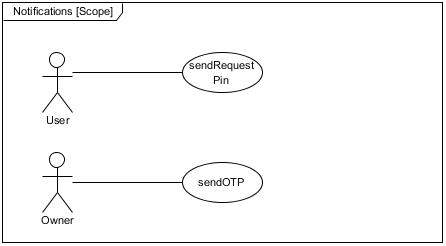
\includegraphics[width=1\textwidth]{./Pictures/UML/notificationsScope.jpg}\\[1.5cm]
	
	{\noindent}The scope of the Notifications module includes
	\begin{itemize}
		\item sending a request for an OTP.
		\item sending the OTP to the user/delivery person.
	\end{itemize}
	
	\newpage
	\subsubsection{Domain Model}
	
	The scope of the Controller module is shown below
	
	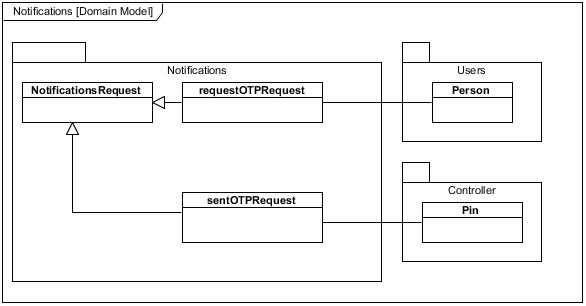
\includegraphics[width=1\textwidth]{./Pictures/UML/notificationsDomainModel.jpg}\\[1.5cm]
	
	{\noindent}\textbf{requestOTP} used by the User/delivery person to request an OTP form the Owner. Message is sent to the Owner which then has to reply with an \textbf{sentOTP}.\\
	
	{\noindent}\textbf{sendOTP} used by the Owner to sent an OTP to the requesting party. In this case it would be a delivery person.\\	 
	
	\subsubsection{Use Cases}
	
	\begin{itemize}
		\item \textbf{sendRequestPin} - User sends a message to the Owner that informs them that a request for an OTP has been made.\\[0.5cm]
		\textit{preconditions:}
		\begin{itemize}
			\item User requires access to the demarcated area.
		\end{itemize}
		
		\textit{postconditions:}
		\begin{itemize}
			\item A pin request message is sent to the Owner.\\[0.5cm]
		\end{itemize}
		
		\item \textbf{sendOTP} - Allows the Owner to send a generated pin to the delivery person.\\[0.5cm]
		\textit{preconditions:}
		\begin{itemize}
			\item The owner has received a pin request from the delivery person.
			\item The requester has authorisation.
			\item a Pin has been generated on the system.
		\end{itemize}
		
		\textit{postconditions:}
		\begin{itemize}
			\item The generated pin is sent to the requester.\\[0.5cm]
		\end{itemize}
	\end{itemize}
	
	\newpage
	\section{Architectural Requirements/Design Specification}
	
	\subsection{Software architecture overview}
	
	The diagram below provides a high-level overview of the software architecture as a whole. For this particular project we are making use of a layered software architecture, therefore the diagram shows how the respective components of the system will be layered.\\
	
	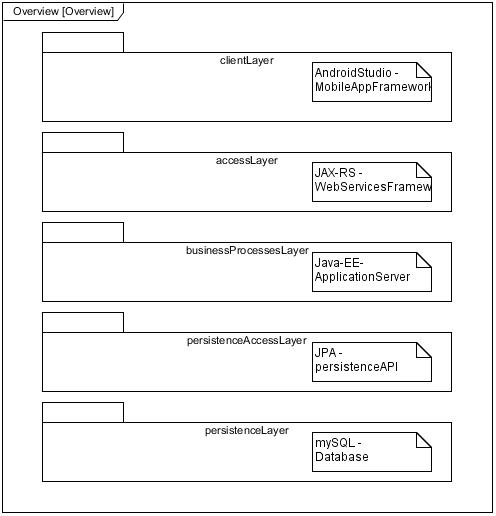
\includegraphics[width=1\textwidth]{./Pictures/UML/architectureOverview.jpg}\\[1.5cm]
	
	
	\subsubsection{clientLayer}
	The layer with which the client will be interacting. This will represent the interface with which the client will be interacting, be it an android or web interface.
	\subsubsection{accessLayer}
	The layer represents the Restful web services layer. It will be used to wrap business process as RESTful services so that multiple access channels may make use of these services. 
	\subsubsection{businessProcessesLayer}
	This layer will host all the business logic within the application server. All methods will be executed server side, and all processes will be hosted on the JBoss server.
	\subsubsection{persistenceAccessLayer}
	This layer represents the Java Persistence API that is used to interact with the database. The client will never interact with the database directly but instead will make use of Entity managers.
	\subsubsection{persistenceLayer}
	This layer refers to the actual database technology that is used for persistence. In this case we will be using a mySQL relational database for persistence.
	
	\subsection{Access Channel Requirements}
	\begin{itemize}
		\item An android application that allows the owner of the property to be notified when someone is outside the premises and to have a full video stream while the person is in the resident.
		
		\item The android application also allows the owner to remotely open and close the premises.
		
		\item The application will also let the owner generate a one-time pin to enable the person to enter the premises (This is the initial system and will be later used as the backup system).  
		
		\item A JFrame touch screen intercom system that allows the delivery person who wants to enter the premises, to enter the pin that was generated by the owner and gain access to the resident.
		
		\item A web application to enable the owner of the property to view recorded camera footage and to configure the camera angles along with system settings. 
	\end{itemize}
	
	\newpage
	\subsection{Architectural Scope}
	\begin{itemize}
		\item Video stream access of the premises from anywhere at any time i.e. constant camera footage of the premises. This will be done using SIP (Session Initiation Protocol).
		
		\item Voice will also be transmitted using SIP, when the delivery person interacts with the intercom system.
		
		\item An internal server that hosts all the devices in the household, allowing for additional devices to be connected at any time. 
		
		\item An external could server to allow communication with the internal server and the android application the owner will be using. 
	\end{itemize}
	
	\subsection{Global Quality Requirements}
	
	\subsubsection{Performance}
	\begin{itemize}
		\item The system has to be stable and responsive enough to send a package with the auto generated pin. The system should also to stable enough to stream video to the android application used by the owner. 
	\end{itemize}
	
	\subsubsection{Security}
	\begin{itemize}
		\item In terms of sending the OTP, end to end encryption with (check best hashing algorithm) will be used. For the initial system (which will be later used as the backup system) the OTP will be sent in a HTTP package. 
		\item The OTP generated will be deleted once used, this ensures that a pin that was used will not work again if the delivery person attempts to use it at a later stage.
		\item In future the system will enforce confidentiality through encrypted communication of SIP (Session Initiation Protocol).
		\item Users of the system will will also need to be authenticated before they may make use of the various processes.
		\item Certain functionality will be restricted to the authorisation of a user, i.e. what role the user has within the system.
	\end{itemize}
	
	\subsubsection{Reliability}
	\begin{itemize}
		\item The property owner should be able to access the residence at any time using the android application 
		\item The user should be able to grant access at any time using the application
		\item With regards to the backup system, the user should be able to generate a pin from anywhere and the pin should work by granting access to the delivery person. 
		\item The response of the gate opening when the user opens it using the application should be reasonable.
	\end{itemize}
	
	\subsubsection{Flexibility}
	\begin{itemize}
		\item The user should be able to access the application from any of his/her devices.
		\item The application should be able to run smoothly on any android device that is Android 4.0 and above.
	\end{itemize}
	
	\subsubsection{Maintainability}
	\begin{itemize}
		\item Maintenance of this application will be handled by the developers, hence the use of an external server.
		\item The server will have to be well maintained because all the people who have this system in their homes will connect to the external server. 
		\item Developers should be able to to add new functionality to the system, as well as change some if the existing functionality if they wish.
	\end{itemize}
	
	\subsubsection{Monitorability}
	\begin{itemize}
		\item While the delivery person is on the premises the owner of the property keeps track of all the activities on the resident. 
		\item When there is no one on the resident, the cameras monitor all movement on the premises.  
	\end{itemize}
	
	\subsubsection{Usability}
	\begin{itemize}
		\item The application should be simple enough for the user to use it without any training. 
		\item The application should have basic instructions to ensure that the user is 100\% sure of the action they are performing.
	\end{itemize}
	
	\subsubsection{Cost}
	\begin{itemize}
		\item The cost of the system should be kept to a minimum and made as affordable as possible. 
		\item This system will mainly use Raspberry pis, keeping the development costs low. 
	\end{itemize}
	
	
	\subsubsection{Testability}
	\begin{itemize}
		\item The individual components of the system needs to be testable through the use of mock objects and automated unit tests.
		\item Automated integration tests should be used to test the system as a whole.
		\item In particular the tests need to verify that the preconditions are met, and that post conditions hold true once a service has been provided.
	\end{itemize}
	
	\subsection{Architectural Constraints}
	The client has some architectural specifications in place that will need to be adhered to, in order to successfully complete this project.
	
	\subsubsection{Use of Inexpensive Devices}
	The devices used to construct the physical system needs to be as inexpensive as possible, thus providing a larger audience with access to it. Devices such as the following will be included:
	\begin{itemize}
		\item Raspberry Pi 3
		\item IP Camera/Pi Camera
		\item Internet Enabled Switches
		\item WiFi Routers
		\item Android Smartphone (Users are assumed to posses one already).
	\end{itemize}
	
	\subsubsection{Technology Stack}
	For monetary reasons, the client has requested that the entire system be developed using open source technologies. CodeBlox has therefore decided to settle on the Java Ecosystem, since we have already had exposure to such technologies. a Preliminary stack will include the following technologies:
	
	\begin{itemize}
		\item \textbf{Java EE} as the primary development platform
		\item \textbf{NetBeans IDE} as the primary development environment.
		\item \textbf{Android Studio} to the build the mobile application that will be used.
		\item \textbf{Apache Maven} will be used as the primary build tool
		\item \textbf{Mockito/TestNG} for unit testing
		\item \textbf{JAX-RS} for implementing RESTful webservices.
		\item \textbf{JBoss} for the primary application server (New version of glassfish seems to have some issues).
		\item \textbf{Linux} as the operating system
		\item \textbf{MySQL} as the primary persistence technology.
	\end{itemize}
	
	\subsection{Architectural Design}
	This section specifies the architectural responsibilities of various architectural components.
	\subsubsection{Architectural Responsibilities}
	\begin{itemize}
		\item The responsibility of providing an execution environment for business processes is assigned to an application server. i.e. \textbf{JBoss}
		\item The responsibility of persisting domain objects is assigned to the the database i.e. \textbf{MySQL}
		\item The responsibility of providing access to the database is assigned to the persistence API i.e. \textbf{Java Persistence API (JPA)}
		\item The responsibility of providing access channels to users is assigned to the web services framework i.e. \textbf{Jersey, which is an implementation of JAX-RS for RESTful Web Services}
		\item The responsibility of providing users access via mobile devices is assigned to the mobile application framework i.e. \textbf{Android Studio}
	\end{itemize}
	
	\subsubsection{Infrastructure}
	For this particular project, the \textbf{layered architectural pattern} will be used as an infrastructure. The pattern limits access of components within one layer to components which are in the same layer or one level down. Thus it cannot access components in the layer above it. What makes it a very useful pattern is that different levels can be easily replaced without disrupting layers either above or below it. 
	
	\newpage
	\subsection{Application Server}
	The application server refers to the architectural component within which business processes are deployed and executed. Put in other words, the application server will be hosting the business processes layer of the system.
	
	\subsubsection{Quality Requirements}
	\begin{itemize}
		\item\textbf{Flexibility}
		\begin{itemize}
			\item deploy different versions of the system with minimum downtime.
		\end{itemize}
		
		\item\textbf{Reliability}
		\begin{itemize}
			\item Requires that service requests are not partially executed. Thus the requested service will only be executed once postconditions are fulfilled. If a service could not be provided, a reason must be given.
		\end{itemize}
		
		\item\textbf{Security}
		\begin{itemize}
			\item The application server must support role-based authorisation. Thus only a user with a certain level of authorisation may execute certain processes. No direct access should be provided to the database. 
		\end{itemize}
		
		\item\textbf{Testability}
		\begin{itemize}
			\item The application server should support out-of-container testing as well as unit testing.
		\end{itemize}
		
	\end{itemize}
	
	\subsubsection{Tactics as provided by Java EE}
	Java EE 7 supports all of the architectural tactics which are specified in the software architecture specific to the application server.
	
	\begin{itemize}
		\item\textbf{Flexibility Tactics}
		\begin{itemize}
			\item Context and Dependency Injection (CDI) is fully supported by Java-EE by using the @Injection annotations.
			\item Hot deployment is supported by the \textbf{JBoss} application server.
		\end{itemize}
		
		\item\textbf{Reliability Tactics}
		\begin{itemize}
			\item Java-EE supports container-managed transactions across multiple transaction-supporting resources. Transaction requirements can be specified by annotating services with TransactionAttribute.Required.
		\end{itemize}
		
		\item\textbf{Security}
		\begin{itemize}
			\item Java-EE supports role-based authorisation in the form of container managed declarative authorisation and programmatic authorisation. Methods are annotated with the required security roles.
		\end{itemize}
		
		\item\textbf{Testability}
		\begin{itemize}
			\item Java-EE supports dependency injection and Java-EE specific information is specified via annotations. All application code can thus be executed outside containers. Dependency injection can be used to inject mock objects allowing unit tests to be reused.
		\end{itemize}
		
	\end{itemize}
	\subsection{Database}
	For this particular project we will be utilising a relational database, namely \textbf{MySQL}. Support for the MySQL database is well documented and most developers are fairly familiar with it and its use. 
	
	\subsection{Persistence API}
	The persistence API will provide indirect access to the MySQL database. For the particular project the Java Persistence API will be used.
	
	{\noindent}JPA implements the following:
	\begin{itemize}
		\item\textbf{object-relational mapping}
		\item\textbf{query mapping}
		\item\textbf{object caching}
		\item\textbf{transaction support}
		\item\textbf{connection pooling}
	\end{itemize}
	
	{\noindent}For all query purposes, the Java Persistence Query Language (JPQL) will be used.
	
	\subsection{Web Services Framework}
	The web services framework refers to a wrapping layer that are used to wrap all business processes. This allows for the decoupling of user-interface technologies (in this case android app or web page) from the back end technologies.
	
	\subsubsection{Architecture Design}
	The project will make use of the Jersey implementation of JAX-RS of the JAVA-EE application server. Marshalling and demarshalling will be achieved by making use of the relevant annotations i.e. @produces and @consumes.
\end{document}
